\chapter{Vorlesung}
\section[Das Heiratsproblem]{Das Heiratsproblem - Maximum cardinality matching in bipartiten Graphen}
\begin{wrapfigure}[5]{L}{0.4\linewidth}
\centering
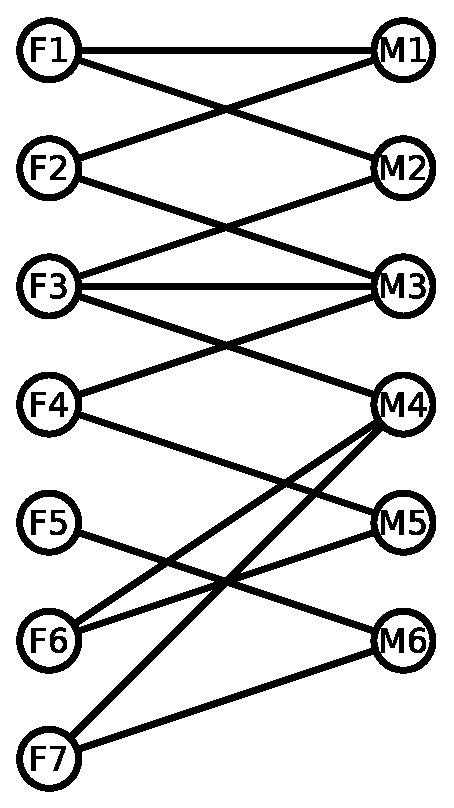
\includegraphics[width=0.5\linewidth]{23/Grafik/Diagramm1}
\caption{Ausgangsproblem}
\label{fig:Diagramm1}
\end{wrapfigure}
\[ G=(V_1 \dot{\cup}V_2, E) \]

$E \subseteq E$ heißt Matching, wenn jeder Knoten zu höchstens einer Kante aus $M$ inzident ist. Freie Knoten sind an keiner Matching-Kante beteiligt.\\

$M$ heißt \underline{maximales} Matching, wenn $M$ durch Hinzunahme einer weiteren Kante nicht vergrößert werden kann.\\

Gesucht ist ein \underline{maximum}-Matching\linebreak[4] $M^*$ mit $|M^*| \geq |M|~\forall~M$ Matching.
\vspace{80pt}

\begin{figure}[H]
	\centering
	\begin{subfigure}[H]{0.4\linewidth}
		\centering
		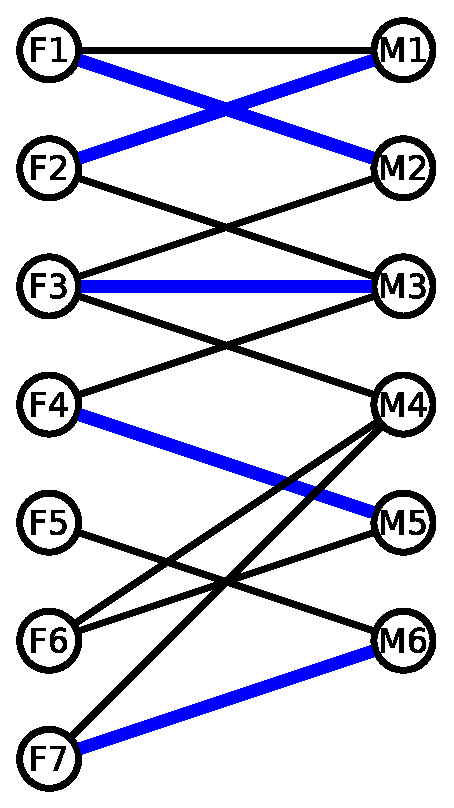
\includegraphics[width=0.5\linewidth]{23/Grafik/Diagramm2}
		\caption{Nicht optimales Matching}
		\label{fig:Diagramm2}
	\end{subfigure}
	\begin{subfigure}[H]{0.4\linewidth}
		\centering
	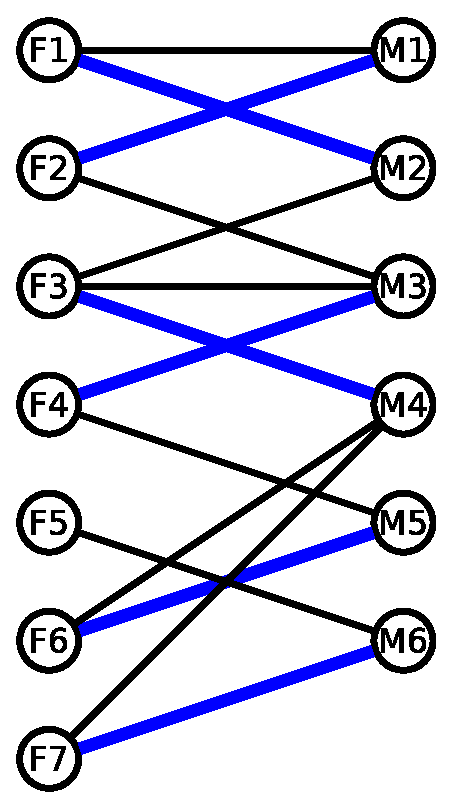
\includegraphics[width=0.5\linewidth]{23/Grafik/Diagramm3}
	\caption{optimales Matching}
	\label{fig:Diagramm3}
	\end{subfigure}
\end{figure}%zu figure ändern und Dia3 hinzufügen
\pagebreak

\begin{wrapfigure}{l}{0.7\linewidth}
	\centering
	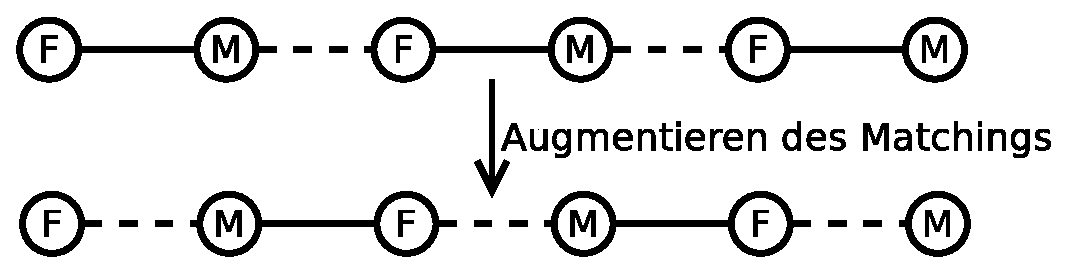
\includegraphics[width=\linewidth]{23/Grafik/Diagramm4}
	\caption{Alternierender Pfad}
	\label{fig:Diagramm4}
\end{wrapfigure}
Alternierender Graph, der mit einem Singleknoten startet und endet, nennt man einen augmentierten Pfad.\\


Zum finden eines augmentierten Pfades verwenden wir folgenden Graphen \\
$G_M = (V_1\cup V_2\cup \{ s \}, E')$
\begin{alignat*}{2} E'= &
\{ (v_1,v_2)|v_1\in V_1, v_2\in V_2, (v_1,v_2)\in E\setminus M \}\\
&\cup\{ (v_2,v_1)|v_1\in V_1, v_2\in V_2, (v_1,v_2)\in M \} \cup \{ (s,v_1)|v_1\in V_1 \text{ frei}\}
 \end{alignat*}
 Mit Hilfe von BFS oder DFS können wir in $G_M$ augmentierende Pfade leicht finden. Also
 \[ \text{Zei } \mathcal{O}(|V|+|E|)\]
 \subsection{Lemma: (Berge)}
 Ein Matching $M$ ist ein maximum-Matching $\Leftrightarrow$ Es gibt keinen $M$-augmentierenden Pfad.
 \subsection{Beweis:}
 \paragraph{"'$A\Rightarrow B$"'}
\begin{description}
 	\item[$\neg B \Rightarrow \neg A$] Es gibt $M$-augmentierenden Pfad $\Rightarrow$ $M$ ist kein maximum Matching
 \end{description}
 \paragraph{"'$A\Leftarrow B$"'}
 \subparagraph{$\neg A \Rightarrow \neg B$}
 Sei $M$ noch kein maximum Matching.
 \subparagraph{z.z.} Es gibt ein $M$-augmentierenden Pfad\\
 $M^*$ sei ein maximum Matching, d.h. $|M^*| > |M|$.\\
 Betrachte den Graphen $\tilde{G} = (V_1\cup V_2, M\oplus M^*)$\\
 Alle Knoten in $\tilde{G}$ haben höchstens Grad 2, ansonsten wäre ein Knoten inzident zu zwei Kanten aus dem Gleichen Matching $M$ oder $M^*$.\\
 $\tilde{G}$ besteht aus einzelnen Knoten, Pfaden gerader oder ungerader Länge und Zyklen gerader Länge.
 \begin{figure}[H]
\centering
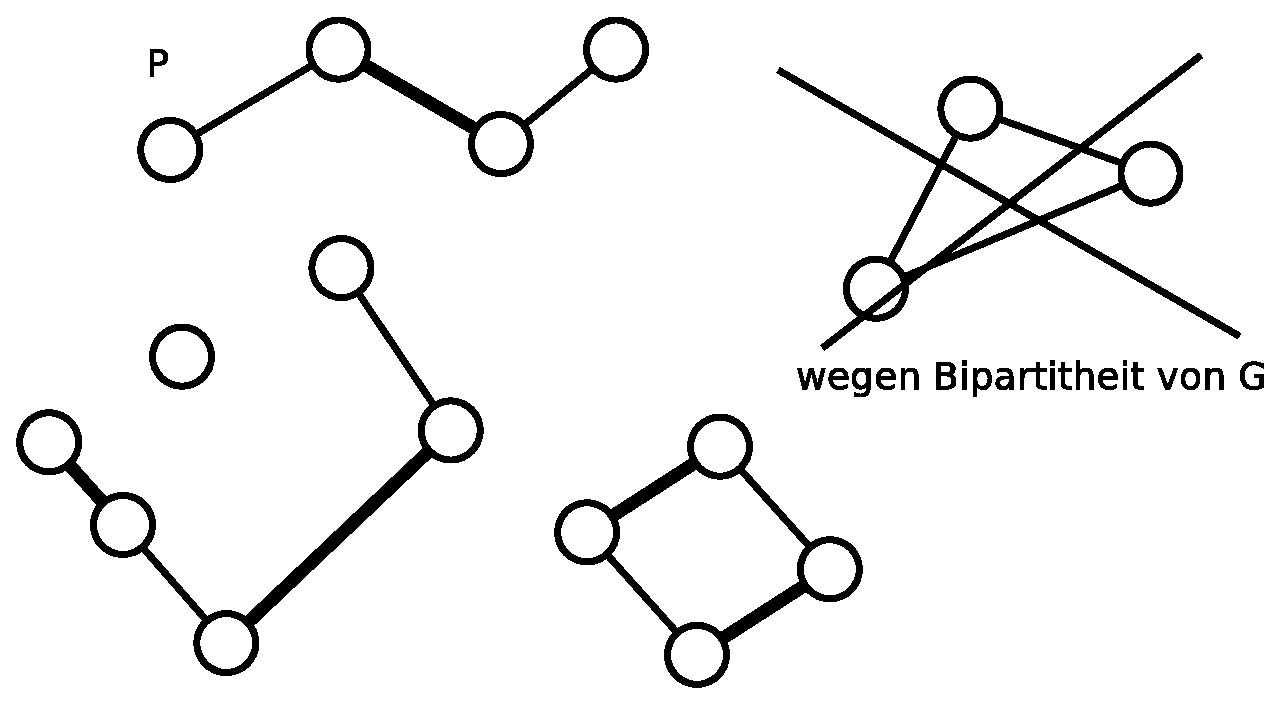
\includegraphics[width=0.3\linewidth]{23/Grafik/Diagramm7}
\caption{Beispiel}
\label{fig:Diagramm7}
\end{figure}

 \subparagraph{z.z.} Es gibt in $\tilde{G}$ mindestens einen $M$-augmentierenden Pfad $p$, der mehr Kanten aus $M^*$ als aus $M$ besitzt. Dies gilt, weil ansonsten $|M^*| \leq |M|$
 \begin{flushright}
 	q.e.d.
 \end{flushright}
 \subsection{Pseudo-Code}
 \begin{lstlisting}
 M = $\emptyset$;
 do {
	 P = findAugmPath($G_M$);
	 if (P == NULL) break;
	 M = M $\oplus$ P;
 } while(true);
 \end{lstlisting}
 \subsubsection{Wiederholung: Symmetrische Differenz}
 \[ A\oplus B = A\setminus B \cup B \setminus A \]
 \begin{figure}[H]
\centering
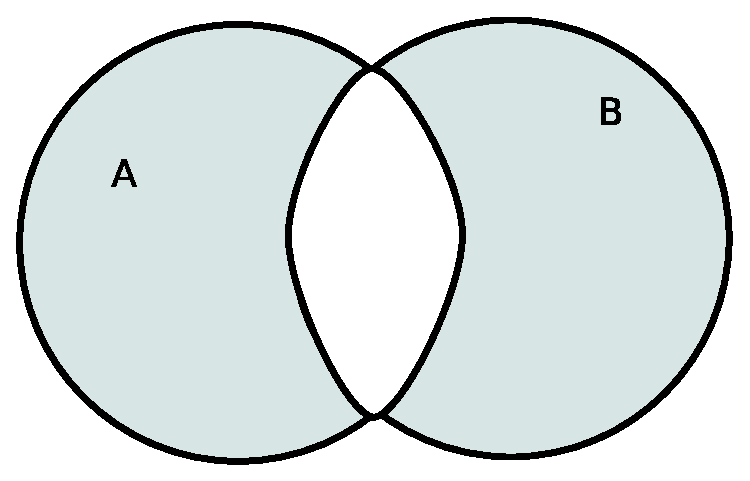
\includegraphics[width=0.3\linewidth]{23/Grafik/Diagramm9}
\caption{Symmetrische Differenz}
\label{fig:Diagramm9}
\end{figure}

 %Grafik9
 \section{Laufzeit}
 \[ \mathcal{O}\left( \min(|V_1|,|V_2|)\cdot(|V|+|E|) \right)\]
 \[ =\mathcal{O}(|V|\cdot|E|) \]
 \section{Hopcroft-Karp-Algorithmus}
 erzielt Laufzeit von $\mathcal{O}(\sqrt{|V|}\cdot |E|)$\\
 \begin{lstlisting}
M = $\emptyset$;
do {
	$G_L$ = buildLevelGraph($G_M$);			//Knotendisjunkte $M$-augmentierende Pfade
	$\mathcal{P}$ = findAugmPath($G_L$);				//$\mathcal{P}=P_1 \dot{\cup}P_2\dot{\cup}\ldots\dot{\cup}P_k$
	M = M $\oplus$ \mathcal{P};
} while($\mathcal{P} \neq \emptyset$);
 \end{lstlisting}
 $G_L$ kann mittels BFS in Zeit $\mathcal{O} (|V|+|E|)$ konstruiert werden. Zum Auffinden einer maximalen Menge von $M$-augmentierenden Pfaden in $G_L$ verwenden wir DFS und entfernen jedes mal den gefunden Pfad $P_i$ aus $G_L$. DFS sorgt dafür, dass $P_i$ in Zeit $\mathcal{O}(|P_i|)$ gefunden und gelöscht werden kann.\\
 $\Rightarrow$ \texttt{findAugmPaths($G_L$)} hat nur Laufzeit $\mathcal{O}(|E|)$